%!TEX root = ../rapport.tex
%!TEX encoding = UTF-8 Unicode

% Chapitres "Introduction"

% modifié par Francis Valois, Université Laval
% 31/01/2011 - version 1.0 - Création du document

\chapter{Avancement de la conception et de la construction du système}
\label{s:avancement}
\section{Alimentation des périphériques 5V}
L'alimentation employée pour les périphériques est une alimentation de type buck qui convert la tension de la batterie (11.1V) vers une tension usuelle de 5V. Cette alimentation utilise un hacheur de tension avec une fréquence autour de 50kHz. Cette fréquence procure une marge de sécurité par rapport à la fréquence d'antenne et évite l'ajout d'un bruit excessif. Cette alimentation a été réalisée avec succès, les plans sont présentés à la figure \ref{fig:alim5V}. Une photo de ladite alimentation est présentée à la figure \ref{fig:alim5Vphoto}.

\begin{figure}[htbp]
\centering
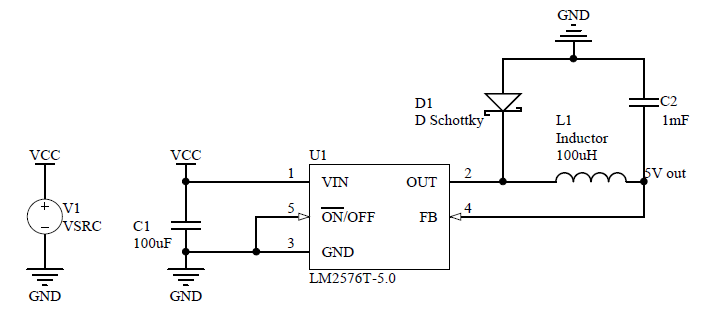
\includegraphics[scale=0.5]{fig/alim_5V.png}
\label{fig:alim5V}
\caption{Figure présentant les plans de l'alimentation 5V pour les périphériques}
\end{figure}

\begin{figure}[htbp]
\centering
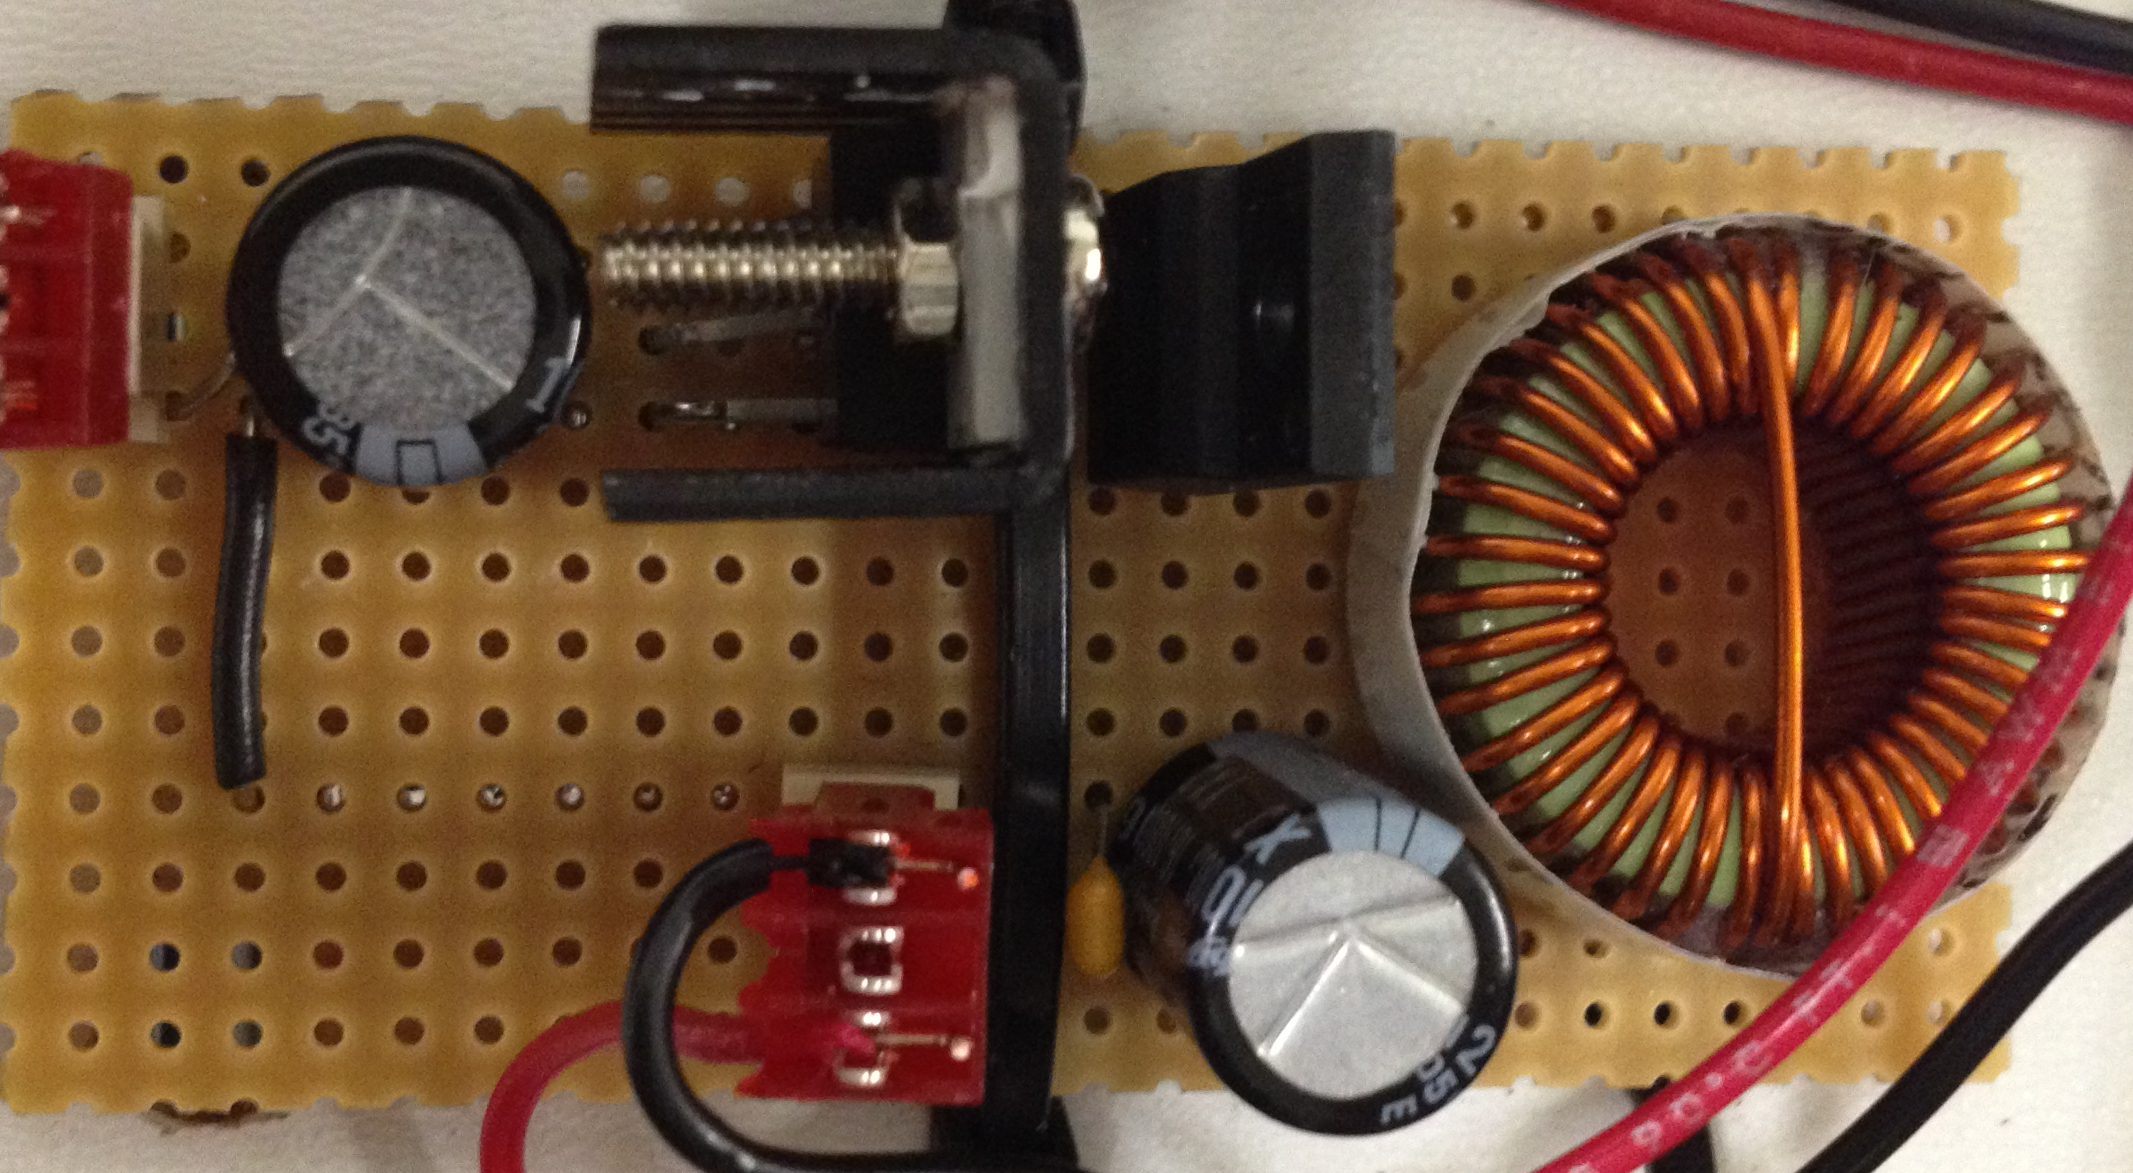
\includegraphics[scale=0.2]{fig/alim_5V_photo.png}
\label{fig:alim5Vphoto}
\caption{Figure présentant une photo de l'alimentation 5V pour les périphériques}
\end{figure}

\section{Alimentation du Mac mini}
L'alimentation du Mac mini a été réalisé au moyen d'un circuit de type Boost réglable, acheté déjà monté. Les plans ne sont pas disponibles, mais une photo du dispositif l'est à la figure \ref{fig:alim24Vphoto}.

\begin{figure}[htbp]
\centering
\includegraphics[scale=0.1]{fig/alim_24V_photo.png}
\label{fig:alim24Vphoto}
\caption{Figure présentant une photo de l'alimentation 24V pour les périphériques}
\end{figure}

\section{Asservissement des moteurs}
\subsection{Modélisation}
L'optimisation des paramètres de réglage a été réalisée grâce à l'utilisation d'un outil de CAO élaboré au moyen de Matlab-Simulink. La fonction de transfert des moteurs a été identifiée au moyen d'une réponse à l'échelon et de l'outil \textit{ident} de Matlab. L'ordre choisi de la fonction est élevé et présente une concordance de 94\% avec la réponse obtenue expérimentalement. L'outil \textit{pidtool} permet par la suite de configurer adéquatement le PIDF et d'obtenir la réponse souhaitée et les paramètres associés. Suivant ces paramètres, le PIDF présent dans le micontrôleur est ajusté.
\paragraph{}L'usage de l'outil interactif permet d'optimiser la réponse et d'obtenir des paramètres de préréglages qui limitent le nombre d'itérations. La réponse obtenue logiciellement est présentée à la figure \ref{fig:as_1}
\begin{figure}[htbp]
\centering
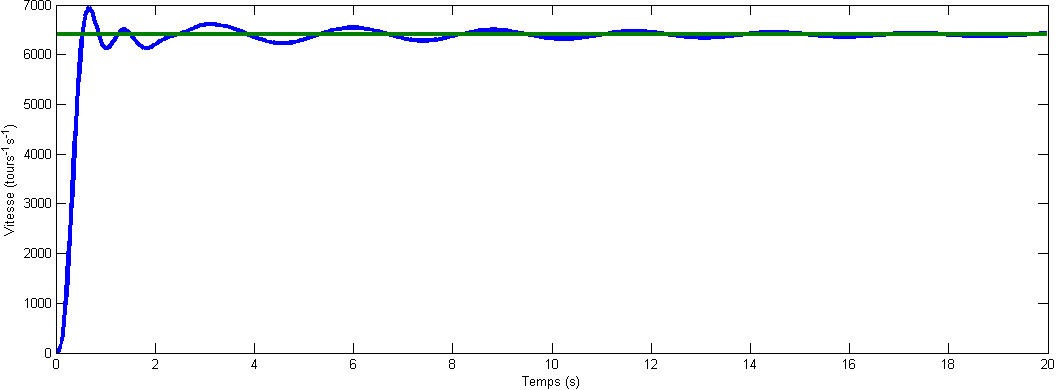
\includegraphics[scale=0.6]{fig/asservissement_1.png}
\label{fig:as_1}
\caption{Figure présentant la réponse à un échelon de consigne de 6400$\left[tours^{-1}s^{-1}\right]$ du système régulé au moyen du régulateur optimisé dans simulink}
\end{figure}
\subsection{Implantation pratique}
La réponse à un échelon de consigne de 6400 ($tours^{-1} s^{-1}$) avec les paramètres de réglage réels est présentée à la figure \ref{fig:as_2}
Le système a été implanté avec un asservissement en vitesse et sans asservissement de position. Les expériences pratiques réalisées montrent que l'évolution de la position est linéaire, et ce, sans asservissement. La figure \ref{fig:as_3} présente ce phénomène pour une consigne de 6400 ($tours^{-1} s^{-1}$) qui vise à amener le système à une position de 9100 $tours^{-1}$.
En utilisant les paramètres obtenus dans Matlab comme point de départ, les paramètres de réglages ont été modifiés de manière à obtenir des réponses remplissant les critères de stabilité, de vitesse et de dépassement souhaités. Afin d'améliorer la vitesse des déplacements, différents PID ont été ajustés selon différentes vitesses d'asservissement. On compte 3 de ces PID pour les déplacements unilatéraux et 1 déplacement réservé pour les mouvements reliés au dessin. La différence est que la vitesse de dessin est beaucoup plus basse que celle du déplacement usuel en vue de permettre une plus grande précision. Le moteur n'étant plus très linéaire à ces faibles vitesses (roulement et zone morte très limitants) et le système étant incapable de démarrer de lui même pour procéder à l'identification, le PID a donc été ajusté de manière manuelle, par itérations. Les PID sont fonctionnels et les systèmes stables, cependant, la décélération avant l'arrêt et le positionnement critique se font par l'entremise d'un palier de ralentissement à une vitesse intermédiaire avant freinage. Ces courbes de décélérations sont à mettre au point avant de pouvoir entamer le contrôle en dessin. Par ailleurs, les mouvements en diagonale ne sont pas encore parfaitement au point et requièrent quelques heures de travail additionnelles.
\begin{figure}[htbp]
\centering
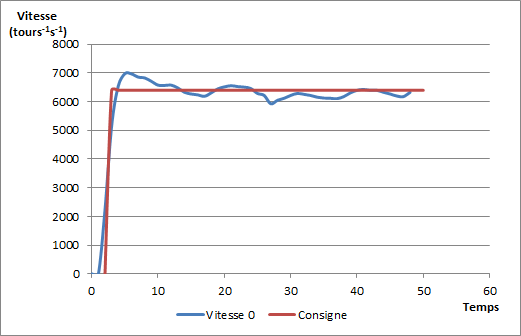
\includegraphics[scale=0.6]{fig/asservissement_3.png}
\label{fig:as_2}
\caption{Figure présentant la réponse à un échelon de consigne de 6400$\left[tours^{-1}s^{-1}\right]$ du système régulé au moyen du régulateur réel et de la réponse en position associée}
\end{figure}
\begin{figure}[htbp]
\centering
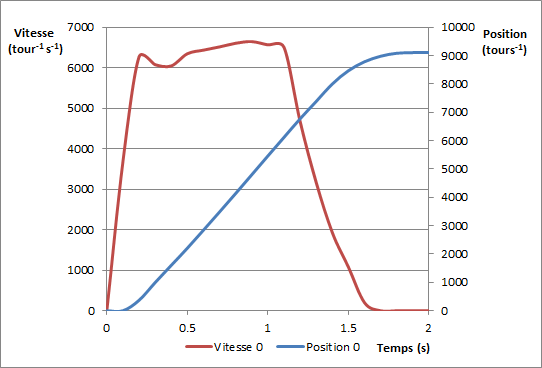
\includegraphics[scale=0.6]{fig/asservissement_2.png}
\label{fig:as_3}
\caption{Figure présentant la réponse à un échelon de consigne de 6400$\left[tours^{-1}s^{-1}\right]$ du système régulé au moyen du régulateur réel et de la réponse en position associée}
\end{figure}
